\documentclass{article}
\usepackage[a4paper, margin=2cm]{geometry}

\usepackage{amsmath}
\usepackage{amssymb}
\usepackage{mathtools}
\usepackage{amstext}
\usepackage{amsthm}
\usepackage{fancyhdr}
\usepackage[utf8]{inputenc} % allow utf-8 input
\usepackage[T1]{fontenc}    % use 8-bit T1 fonts
\usepackage{simpler-wick}

\usepackage{graphicx}
\usepackage{float}
\usepackage{caption}
\usepackage{subcaption}
\usepackage{booktabs}
\usepackage{physics, tensor}
\usepackage{slashed, cancel}

\graphicspath{{figures/}}

\pagestyle{fancy}
\rhead{Alexandre Adam\\ 20090755}
\lhead{William Witczak-Krempa \\ PHY 6812: Théorie des champs 1}
\chead{Devoir 5}
\rfoot{14 décembre 2022}
\cfoot{\thepage}

\newcommand{\angstrom}{\textup{\AA}}
\numberwithin{equation}{section}
\renewcommand\thesubsection{\alph{subsection})}
\renewcommand\thesubsubsection{\Roman{subsubsection}}
\newcommand{\s}{\hspace{0.1cm}}
\DeclareRobustCommand{\bbzero}{\text{\usefont{U}{bbold}{m}{n}0}}
\DeclareRobustCommand{\bbone}{\text{\usefont{U}{bbold}{m}{n}1}}


\theoremstyle{solution}
\newtheorem{solution}{Réponse}[section]
\newtheorem*{solution*}{Réponse}

\renewcommand*{\proofname}{Solution}


\begin{document}

\section{Fonction de corrélation pour QFT scalaire interagissante $\phi^{4}$}
\begin{solution*}
La fonction de corrélation à trois points est nulle dans la théorie interagissante $\phi^{4}$
       \begin{equation}
               \langle \Omega | T \left\{ \phi(x_{1}) \phi(x_2) \phi(x_3) \right\} | \Omega \rangle  = 0\, ,
       \end{equation}
       où $\phi(x)$ est un opérateur de champs Klein-Gordon dans le point de vue d'Heisenberg.
\end{solution*}
\begin{proof}
Par définition, la fonction de corrélation à trois points dans la théorie interagissante $\phi^{4}$ en $(d+1)$ dimensions prend la forme
\begin{equation}
        \langle \Omega | T \{\phi(x_1) \phi(x_2) \phi(x_3) | \Omega \} \rangle = \lim\limits_{T \rightarrow  \infty (1 - i \epsilon)}
        \dfrac{\langle 0 | T \{\phi_{I}(x_{1}) \phi_{I}(x_2) \phi_{I}(x_3) 
        \exp \left( -i \int_{-T}^{T} dt\, \int d^{3}\mathbf{z}\, \frac{\lambda}{4!}\phi_{I}^{4}(t, \mathbf{z}) \right) \} | 0\rangle }
        {\langle 0 | T \{\exp \left( -i \int_{-T}^{T} dt\, \int d^{3}\mathbf{z}\, \frac{\lambda}{4!}\phi_{I}^{4}(t, \mathbf{z})\right) \} | 0 \rangle }\, ,
\end{equation} 
où $\phi_{I}(x)$ est dans la représentation d'interaction. On se concentre maintenant sur le numérateur. Dans la dérivation, 
la limite sur $T$ est implicitement définie dans les bornes de l'intégrale sur l'espace-temps $\int d^{4}z$. Le développement 
de la série de Dyson nous permet d'écrire
\begin{equation}
        \langle \Omega | T \{\phi(x_1) \phi(x_2) \phi(x_3) | \Omega \} \propto 
        \langle 0 | 
        T \left\{  
        \begin{aligned}
        &\phi_{I}(x_1) \phi_I(x_2) \phi_I(x_3) \\
                + &\phi_I(x_1) \phi_I(x_2) \phi_I(x_3) \frac{(-i)\lambda}{4!}\int d^{4}z\, \phi_I^{4}(z) \\
                + &\phi_I(x_1) \phi_I(x_2) \phi_I(x_3) \frac{(-i)^{2}\lambda^{2}}{2!4!}\int d^{4}z\, \phi_I^{4}(z) \int d^{4}w\, \phi_{I}^{4}(w) \\
                + & \dots
        \end{aligned}
\right\} 
        | 0\rangle 
\end{equation} 
On peut évaluer chaque terme à l'aide du théorème de Wick. Le premier terme devient
\begin{align}
        \langle 0 |T \{\phi_{I}(x_1) \phi_I(x_2) \phi_I(x_3)\} | 0 \rangle &=  \langle 0 | :\phi_I(x_1) \phi_I(x_2) \phi_I(x_3) + 
        \begin{pmatrix}
                \text{Toutes les } \\
                \text{contractions possibles}
        \end{pmatrix}
        : 
        | 0 \rangle \\
        &= 0
\end{align} 
En effet, il n'est pas possible de faire une contraction complète pour un nombre impaire d'opérateurs. On peut démontrer explicitement 
ce fait pour le cas $m=3$
\begin{align*}
        :         
        \begin{pmatrix}
                \text{Toutes les } \\
                \text{contractions possibles}
        \end{pmatrix}
        :
        &=\,\, :\wick{\c1 \phi_I(x_1) \c1 \phi_I(x_2) \phi_I(x_3)} +  \wick{\c1 \phi_I(x_1)  \phi_I(x_2) \c1 \phi_I(x_3)} +  \wick{\phi_I(x_1)  \c1 \phi_I(x_2) \c1 \phi_I(x_3)}:
\end{align*}
Dans tous les cas, il reste au moins un opérateur $\phi_{I}(x)$ tels que $\langle 0 | : \phi_{I}(x) : | 0 \rangle  = 0$. Comme chaque terme 
dans le développement de la série de Dyson du numérateur possède strictement un nombre impaire d'opérateur ($m = 3 + 4n$, $n \in \mathbb{N}_0$), alors
\begin{equation}
       \langle 0 | T \{\phi_{I}(x_{1}) \phi_{I}(x_2) \phi_{I}(x_3) 
       \exp \left( -i  \int d^{4}z\, \frac{\lambda}{4!}\phi_{I}^{4}(z) \right) \} | 0\rangle  = 0
\end{equation}  
D'un autre côté, le dénominateur possède toujours un nombre paire d'opérateurs ($m = 4n$, $n \in \mathbb{N}_0$). Donc, 
\begin{equation}
       \langle 0 | T \{\exp \left( -i \int d^{4}z\,  \frac{\lambda}{4!}\phi_{I}^{4}(z)\right) \} | 0 \rangle \not= 0 
\end{equation} 
Ainsi, 
\begin{equation}
        \langle \Omega | T \{\phi(x_1) \phi(x_2) \phi(x_3) | \Omega \} = 0
\end{equation} 
        
\end{proof}
\pagebreak
\section{Fonction de corrélation pour QFT scalaire interagissante $\phi^{3}$}
On considère le terme d'interaction
\begin{equation}
        \hat{H}_{\mathrm{int}} = \int d^{3}\mathbf{x}\, \frac{\lambda}{3!} \hat{\phi}^{3}(\mathbf{x})
\end{equation} 

\subsection{}
On cherche à déterminer
\begin{equation}
       \mathcal{A}(x, y) = \lim\limits_{T \rightarrow  \infty (1 - i \epsilon)}\langle 0 | T \{ \phi(x) \phi(y) \exp \left( -i \int_{-T}^{T} dt\, \hat{H}_{\mathrm{int}}(t) \right) \} | 0 \rangle \, ,
\end{equation} 
à l'ordre $\lambda^{2}$ inclusivement, où $\phi(x)$ est un opérateur de champs Klein-Gordon dans la représentation d'interaction. Le développement 
de la série de Dyson à l'ordre $\lambda^{2}$ est
\begin{equation}
        \mathcal{A}(x, y) = \langle 0 | T \{\phi(x) \phi(y)\} 0 \rangle 
        +\frac{1}{2!} \left(\frac{-i\lambda}{ 3!}\right)^{2} \langle 0 | T \{\phi(x) \phi(y)  \int d^{4}z\, \phi^{3}(z)\, \int d^{4}w\, \phi^{3}(w) \} | 0 \rangle 
        + \mathcal{O}(\lambda^{4})\, .
\end{equation} 
Les termes d'ordre $\lambda^{2n + 1}$, $n \in \mathbb{Z}_{0}$, s'annulent puisqu'ils contiennent un nombre impaire de champs $\phi$.
Le premier terme est simplement $D_{F}(x - y)$. Le second terme, par le théorème de Wick, est la somme des contractions complètes 
de $m = 8$ opérateurs de champs. Au total, il y a $(m - 1)!! = 105$ contractions complètes possibles. Or la plupart de ces contractions sont 
redondantes. 

\paragraph{Les graphes connectés à 4 sommets} On commence par énumérer les graphes connectés à 4 sommets, 
soit deux sommets qui correspondent aux points externes $x$ et $y$, et deux sommets qui correspondent
aux points internes $z$ et $w$. Chacun de ces graphes possède 4 liens, ou propagateurs, correspondants à 4 contractions de 8 opérateurs. 
On peut énumérer les graphes connectés à 4 sommets uniques à partir des symétries des contractions. Pour simplifier la notation, on va simplement écrire
\begin{equation}
        \phi(x) \phi(y) \phi(z)\phi(z)\phi(z)\phi(w) \phi(w) \phi(w) = \phi\phi\,\, \phi\phi\phi\,\, \phi \phi \phi 
\end{equation} 
Les sommets $z$ et $w$ sont symétriques, de sortes que certains graphes sont équivalents par échange des sommets. Par exemple, les contractions 
suivantes sont congruentes
\begin{equation}\label{eq:congruence}
        \wick{\c1 \phi \c2 \phi \,\, \c1 \phi \c3 \phi \c4 \phi \, \, \c4 \phi \c3 \phi \c2 \phi} \cong \wick{\c1 \phi \c2 \phi \,\, \c2 \phi \c3 \phi \c4 \phi \, \, \c4 \phi \c3 \phi \c1 \phi} 
\end{equation}
puisqu'elles correspondent à l'échange de deux sommets internes du graphe
\begin{figure}[H]
        \centering
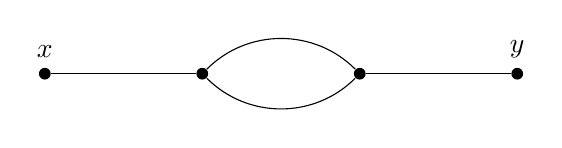
\begin{tikzpicture}
        \node[circle, fill=black, inner sep=1.5pt, label=above:{$x$}] (x) at (-3, 0) {};
        \node[circle, fill=black, inner sep=1.5pt] (z) at (-1, 0) {};
        \node[circle, fill=black, inner sep=1.5pt] (w) at (1, 0) {};
        \node[circle, fill=black, inner sep=1.5pt, label=above:{$y$}] (y) at (3, 0) {};
        \draw (x) edge (z);
        \draw (w) edge (y);
        \draw[out=45, in=135] (z) edge (w);
        \draw[out=-45, in=-135] (z) edge (w);
\end{tikzpicture}        
\end{figure}
\noindent
Ce graphe possède un facteur de symétrie $S = 2$ puisqu'il est possible d'échanger les deux liens entre $z$ et $w$.
En effet, par le théorème de Wick, on peut compter le nombre de contractions congruentes 
à $ \wick{\c1 \phi \c2 \phi \,\, \c1 \phi \c3 \phi \c4 \phi \, \, \c4 \phi \c3 \phi \c2 \phi} $ de la façon suivante:
\begin{equation}
        \underbrace{2!}_{\substack{\text{Échange des} \\ \text{sommets internes}}} \times
        \underbrace{3!}_{\substack{\text{Placement des} \\ \text{contractions pour $z$}}} \times 
        \underbrace{3}_{\substack{\text{Placement des} \\ \text{contractions pour $w$}}} 
        %\underbrace{\frac{1}{2}}_{\substack{\text{Échange des} \\ \text{contractions entre} \\ \text{$z$ et $w$}}}
\end{equation} 
Ainsi, le préfacteur de ce graphe dans le développement de la série de Dyson sera 
\begin{equation}
        \frac{2! \cdot 3! \cdot 3}{2!\cdot 3! \cdot 3!} = \frac{1}{2} = \frac{1}{S}
\end{equation} 
Dans ce qui suit, on déduit simplement le facteur de symétrie par la structure du graphe.
On peut ensuite construire le graphe suivant
\begin{figure}[H]
\centering
\begin{tikzpicture}
        \node[circle, fill=black, inner sep=1.5pt, label=above:{$x$}] (x) at (-2, 0) {};
        \node[circle, fill=black, inner sep=1.5pt] (z) at (0, 0) {};
        \node[circle, fill=black, inner sep=1.5pt] (w) at (0, -1) {};
        \node[circle, fill=black, inner sep=1.5pt, label=above:{$y$}] (y) at (2, 0) {};

        \draw (x) edge (z);
        \draw (z) edge (y);
        \draw (z) edge (w);
        \draw (0, -1.5) circle (.5);
\end{tikzpicture} 
\end{figure}
\noindent
Ce graphe est associé aux contractions congruentes à $\wick{\c1 \phi \c2 \phi \,\, \c1 \phi \c3 \phi \c2 \phi\,\, \c3 \phi \c4 \phi \c4 \phi}$. Ce graphe possède un facteur de symétrie 
$S = 2 $, soit un facter $2$ qui correspond à la boucle fermée. 
Finalement, on peut construire un dernier graphe où $x$ et $y$ sont déconnectés l'un de l'autre, 
mais qui est tout de même considérés comme \textit{connecté} puisqu'il ne contient pas de boucle du vide fermée et déconnectée des points externes. 
\begin{figure}[H]
\centering
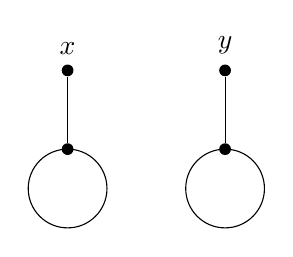
\begin{tikzpicture}
        \node[circle, fill=black, inner sep=1.5pt, label=above:{$x$}] (x) at (-1, 0) {};
        \node[circle, fill=black, inner sep=1.5pt] (z) at (-1, -1) {};
        \node[circle, fill=black, inner sep=1.5pt] (w) at (1, -1) {};
        \node[circle, fill=black, inner sep=1.5pt, label=above:{$y$}] (y) at (1, 0) {};

        \draw (x) edge (z);
        \draw (y) edge (w);
        \draw (1, -1.5) circle (.5);
        \draw (-1, -1.5) circle (.5);
\end{tikzpicture} 
\end{figure}
\noindent
Ce graphe correspond aux contractions congruentes avec $\wick{\c1 \phi \c2 \phi\,\, \c1 \phi \c3 \phi \c3 \phi\,\, \c2 \phi \c4 \phi \c4 \phi}$, et possède un facteur de symétrie 
$S = 4$, qui correspond à la présence de deux boucles fermées.

\paragraph{Les graphes connectés à 3 sommets} On considère maintenant les graphes avec 3 sommets, soit deux points externes et un point interne. 
Dans une théorie $\phi^{3}$, il n'y a pas de graphes connectés à 3 sommets. En effet, une boucle du vide simple pour un terme à trois champs, par exemple $\wick{\phi \c1 \phi \c1 \phi}$, 
doit toujours inclure une contraction avec un champ associé à un autre point, donc il n'est pas possible d'isoler un sommet du graphe.
%\begin{figure}[H]
        %\centering
%\begin{tikzpicture}
        %\node at (-4, 0) {$\wick{\c1 \phi \c2 \phi\,\, \c1 \phi \c2 \phi \c3 \phi\,\, }$}
        %\node[circle, fill=black, inner sep=1.5pt, label=above:{$x$}] (x) at (-2, 0) {};
        %\node[circle, fill=black, inner sep=1.5pt] (z) at (0, 0) {};
        %\node[circle, fill=black, inner sep=1.5pt, label=above:{$y$}] (y) at (2, 0) {};

        %\draw (x) edge (z);
        %\draw (z) edge (y);
        %\draw (0, .5) circle (.5);
%\end{tikzpicture}
%\end{figure}

\paragraph{Les graphes connectés à 2 sommets} On considère maintenant les graphes avec 2 sommets, soit deux points externes. Trivialement, il n'y a qu'un seul graphe avec deux 
sommets externes, soit
\begin{figure}[H]
        \centering
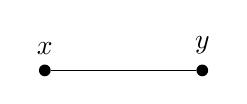
\begin{tikzpicture}
        \node[circle, fill=black, inner sep=1.5pt, label=above:{$x$}] (x) at (0, 0) {};
        \node[circle, fill=black, inner sep=1.5pt, label=above:{$y$}] (y) at (2, 0) {};
        \draw (x) edge (y);
\end{tikzpicture}
\end{figure}
\noindent
qui correspond à la contraction $\wick{\c1 \phi \c1 \phi}$, avec un facteur de symétrie $S = 1$.

\paragraph{Les graphes déconnectés} On énumère finalement les graphes déconnectés. Tels que mentionné précédemment, il ne peut pas y avoir de 
graphe déconnecté à 1 sommet. À l'ordre $\lambda^{2}$, on a seulement les boucles fermées avec $2$ sommets internes et $3$ liens. 
\begin{figure}[H]
        \centering
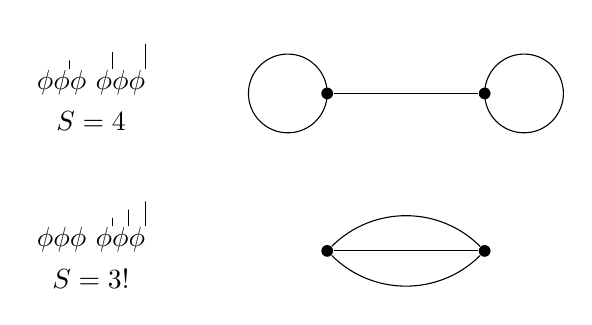
\begin{tikzpicture}
        \node[circle, fill=black, inner sep=1.5pt] (z) at (0, 0) {};
        \node[circle, fill=black, inner sep=1.5pt] (w) at (2, 0) {};
        \draw (z) edge (w);
        \draw (2.5, 0) circle (.5);
        \draw (-.5, 0) circle (.5);
        \node at (-3, .35) {$\wick{\c1 \phi \c1 \phi \c2 \phi \,\, \c2 \phi \c3 \phi \c3 \phi}$};
        \node at (-3, -.35) {$S = 4$};

        \begin{scope}[shift={(0, -2)}]
        \node[circle, fill=black, inner sep=1.5pt] (z) at (0, 0) {};
        \node[circle, fill=black, inner sep=1.5pt] (w) at (2, 0) {};
        \draw[out=45, in=135] (z) edge (w);
        \draw[out=-45, in=-135] (z) edge (w);
        \draw (z) edge (w);
        \node at (-3, .35) {$\wick{\c1 \phi \c2 \phi \c3 \phi \,\, \c1 \phi \c2 \phi \c3 \phi}$};
        \node at (-3, -.35) {$S = 3!$};
        \end{scope}
\end{tikzpicture}
\end{figure}
\noindent
L'échange possibles de 3 liens entre $z$ et $w$ produit un facteur de symétrie $S = 3!$. En effet, par le théorème de Wick on a que
le nombre de contractions congruentes à $\wick{\c1 \phi \c2 \phi \c3 \phi \,\, \c1 \phi \c2 \phi \c3 \phi}$ est
\begin{equation}
        \underbrace{2!}_{\substack{\text{Échange des} \\ \text{sommets internes}}} \times
        \underbrace{3!}_{\substack{\text{Placement des} \\ \text{contractions pour $w$}}}\
\end{equation} 
d'où le préfacteur
\begin{equation}
        \frac{2! \cdot 3!}{2! \cdot 3! \cdot 3!} = \frac{1}{3!} = \frac{1}{S}
\end{equation} 

En collectant tous ces graphes, on obtient le terme suivant
\begin{equation}
\begin{aligned}
        \mathcal{A}(x, y) &= D_F(x - y) + (-i \lambda)^{2} \Biggl( 
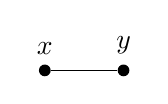
\begin{tikzpicture}[baseline={([yshift=-.5ex]current bounding box.center)}, scale=0.5]
        \node[circle, fill=black, inner sep=1.5pt, label=above:{$x$}] (x) at (0, 0) {};
        \node[circle, fill=black, inner sep=1.5pt, label=above:{$y$}] (y) at (2, 0) {};
        \draw (x) edge (y);
\end{tikzpicture}
\Biggl(
\,\,
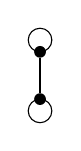
\begin{tikzpicture}[baseline={([yshift=-.5ex]current bounding box.center)}, scale=0.3]
\begin{scope}[rotate=90]
        \node[circle, fill=black, inner sep=1.5pt] (z) at (0, 0) {};
        \node[circle, fill=black, inner sep=1.5pt] (w) at (2, 0) {};
        \draw (z) edge (w);
        \draw (2.5, 0) circle (.5);
        \draw (-.5, 0) circle (.5);
\end{scope}
\end{tikzpicture}
+
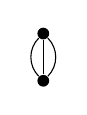
\begin{tikzpicture}[baseline={([yshift=-.5ex]current bounding box.center)}, scale=0.3]
\begin{scope}[shift={(1, 0)}]
        \node[circle, fill=black, inner sep=1.5pt] (z) at (0, 0) {};
        \node[circle, fill=black, inner sep=1.5pt] (w) at (0, 2) {};
        \draw[out=45, in=-45] (z) edge (w);
        \draw[out=135, in=-135] (z) edge (w);
        \draw (z) edge (w);
\end{scope}
\end{tikzpicture}
\Biggl)\\
&\hspace{1cm}+ 
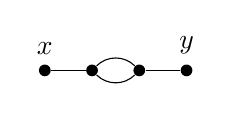
\begin{tikzpicture}[baseline={([yshift=-.5ex]current bounding box.center)}, scale=0.3]
        \node[circle, fill=black, inner sep=1.5pt, label=above:{$x$}] (x) at (-3, 0) {};
        \node[circle, fill=black, inner sep=1.5pt] (z) at (-1, 0) {};
        \node[circle, fill=black, inner sep=1.5pt] (w) at (1, 0) {};
        \node[circle, fill=black, inner sep=1.5pt, label=above:{$y$}] (y) at (3, 0) {};
        \draw (x) edge (z);
        \draw (w) edge (y);
        \draw[out=45, in=135] (z) edge (w);
        \draw[out=-45, in=-135] (z) edge (w);
\end{tikzpicture}        
+
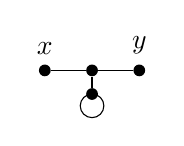
\begin{tikzpicture}[baseline={([yshift=-.5ex]current bounding box.center)}, scale=0.3]
        \node[circle, fill=black, inner sep=1.5pt, label=above:{$x$}] (x) at (-2, 0) {};
        \node[circle, fill=black, inner sep=1.5pt] (z) at (0, 0) {};
        \node[circle, fill=black, inner sep=1.5pt] (w) at (0, -1) {};
        \node[circle, fill=black, inner sep=1.5pt, label=above:{$y$}] (y) at (2, 0) {};

        \draw (x) edge (z);
        \draw (z) edge (y);
        \draw (z) edge (w);
        \draw (0, -1.5) circle (.5);
\end{tikzpicture} 
+
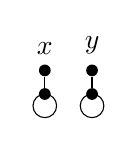
\begin{tikzpicture}[baseline={([yshift=-.5ex]current bounding box.center)}, scale=0.3]
        \node[circle, fill=black, inner sep=1.5pt, label=above:{$x$}] (x) at (-1, 0) {};
        \node[circle, fill=black, inner sep=1.5pt] (z) at (-1, -1) {};
        \node[circle, fill=black, inner sep=1.5pt] (w) at (1, -1) {};
        \node[circle, fill=black, inner sep=1.5pt, label=above:{$y$}] (y) at (1, 0) {};

        \draw (x) edge (z);
        \draw (y) edge (w);
        \draw (1, -1.5) circle (.5);
        \draw (-1, -1.5) circle (.5);
\end{tikzpicture} 
\Biggl)
\,
+\,\, \mathcal{O}(\lambda^{4})
\end{aligned}
\end{equation} 
En collectant les facteur de symétrie pour chaque graphe, on obtient finalement l'amplitude en 
terme des propagateurs de Feynman
\begin{equation}
        \boxed{
\begin{aligned}
        \mathcal{A}(x, y) &= D_F(x - y)  
         + (-i \lambda)^{2}
        \int d^{4}z \, \int d^{4}w
        \bigg( 
        \frac{1}{4}D_F(x - y)D_F(z)D_F(w)D_F(z - w) \\
        &\hspace{1cm}+ \frac{1}{3!}D_F(x - y)D_F^3(z - w) 
        +\frac{1}{2}D_F(x - z)D_F^{2}(z - w)D_F(y - w) \\
        &\hspace{1cm}+\frac{1}{2} D_{F}(x - z)D_F(z - w)D_F(w)D_F(y - z)
       + \frac{1}{4}D_F(x - z)D_F(z)D_F(w)D_F(y - w)
\bigg)
+ \mathcal{O}(\lambda^{4})
\end{aligned}
}
\end{equation} 

\subsection{}
On cherche à déterminer
\begin{equation}
        \mathcal{B} = \langle 0 |T \{ \exp \left( -i \int_{-\infty }^{\infty }\hat{H}_{\mathrm{int}}(t) dt \right)\}  | 0 \rangle 
\end{equation} 
à l'ordre $\lambda^{2}$. On a déjà trouver les bulles du vides qui contribuent à ce processus à l'ordre $\lambda^{2}$. Il n'y a pas 
graphes à l'ordre $\lambda$ pour une théorie $\phi^{3}$. Ainsi, 
\begin{equation}
        \mathcal{B} = 1 + (-i\lambda)^{2} \left( 
\,\,
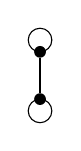
\begin{tikzpicture}[baseline={([yshift=-.5ex]current bounding box.center)}, scale=0.3]
\begin{scope}[rotate=90]
        \node[circle, fill=black, inner sep=1.5pt] (z) at (0, 0) {};
        \node[circle, fill=black, inner sep=1.5pt] (w) at (2, 0) {};
        \draw (z) edge (w);
        \draw (2.5, 0) circle (.5);
        \draw (-.5, 0) circle (.5);
\end{scope}
\end{tikzpicture}
+
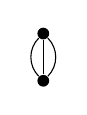
\begin{tikzpicture}[baseline={([yshift=-.5ex]current bounding box.center)}, scale=0.3]
\begin{scope}[shift={(1, 0)}]
        \node[circle, fill=black, inner sep=1.5pt] (z) at (0, 0) {};
        \node[circle, fill=black, inner sep=1.5pt] (w) at (0, 2) {};
        \draw[out=45, in=-45] (z) edge (w);
        \draw[out=135, in=-135] (z) edge (w);
        \draw (z) edge (w);
\end{scope}
\end{tikzpicture}
 \right)
 + \mathcal{O}(\lambda^{4})
\end{equation} 
D'où
\begin{equation}
        \boxed{\mathcal{B} = 1 + (-i\lambda)^{2}\int d^{4}z \int d^{4}w \left( \frac{1}{4}D_F(z - w)D_F(z)D_F(w) + \frac{1}{3!}D_F^{3}(z - w) \right)}
\end{equation} 

\subsection{}
On cherche à calculer
\begin{equation}
        \mathcal{C}(x, y, z) = \langle \Omega |T \{\phi(x) \phi(y) \phi(z)\}  | \Omega \rangle 
\end{equation} 
à l'ordre $\lambda$ inclusivement. On commence par utiliser la représentation d'interactions pour 
l'Hamiltonien de Klein-Gordon avec un terme d'interaction $\phi^{3}$, $\hat{H} = \hat{H_{0}} + \hat{H}_{\mathrm{int}}$.
On assume, sans perte de généralité, que $x^{0} > y^{0} > z^{0}$.
Le terme $\lambda^{0}$ ne contribue pas à $\mathcal{C}$. Pour le terme à l'ordre $\lambda$, on a les graphes suivants qui contribuent
\begin{figure}[H]
\centering
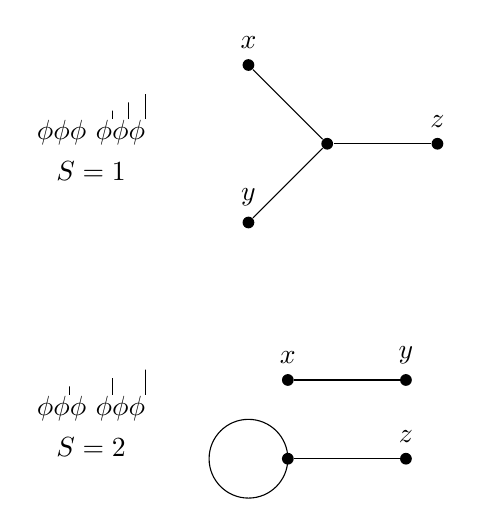
\begin{tikzpicture}
        \node at (-3, 0.35) {$\wick{\c1 \phi \c2 \phi \c3 \phi \,\, \c1 \phi \c2 \phi \c3 \phi}$};
        \node at (-3, -0.35) {$S = 1$};
        \node[circle, fill=black, inner sep=1.5pt, label=above:{$x$}] (x) at (-1, 1) {};
        \node[circle, fill=black, inner sep=1.5pt, label=above:{$y$}] (y) at (-1, -1) {};
        \node[circle, fill=black, inner sep=1.5pt, label=above:{$z$}] (z) at (1.4, 0) {};
        \node[circle, fill=black, inner sep=1.5pt] (w) at (0, 0) {};
        \draw (x) edge (w);
        \draw (y) edge (w);
        \draw (z) edge (w);
        
        \begin{scope}[shift={(0, -3.5)}]
        \node at (-3, 0.35) {$\wick{\c1 \phi \c1 \phi \c2 \phi \,\, \c2 \phi \c3 \phi \c3 \phi}$};
        \node at (-3, -0.35) {$S = 2$};
        \node[circle, fill=black, inner sep=1.5pt, label=above:{$x$}] (x) at (-.5, .5) {};
        \node[circle, fill=black, inner sep=1.5pt, label=above:{$y$}] (y) at (1, .5) {};
        \node[circle, fill=black, inner sep=1.5pt, label=above:{$z$}] (z) at (1, -0.5) {};
        \node[circle, fill=black, inner sep=1.5pt] (w) at (-.5, -0.5) {};
        \draw (x) edge (y);
        \draw (w) edge (z);
        \draw (-1, -0.5) circle (0.5);
        \end{scope}
\end{tikzpicture}
\end{figure}
\begin{equation}
        \boxed{
        \begin{aligned}
                \mathcal{C}(x, y, z) &= -i\lambda \left( 
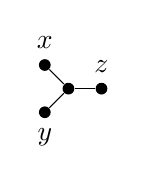
\begin{tikzpicture}[baseline={([yshift=-.5ex]current bounding box.center)}, scale=0.3]
        \node[circle, fill=black, inner sep=1.5pt, label=above:{$x$}] (x) at (-1, 1) {};
        \node[circle, fill=black, inner sep=1.5pt, label=below:{$y$}] (y) at (-1, -1) {};
        \node[circle, fill=black, inner sep=1.5pt, label=above:{$z$}] (z) at (1.4, 0) {};
        \node[circle, fill=black, inner sep=1.5pt] (w) at (0, 0) {};
        \draw (x) edge (w);
        \draw (y) edge (w);
        \draw (z) edge (w);
\end{tikzpicture}
+ 
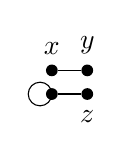
\begin{tikzpicture}[baseline={([yshift=-.5ex]current bounding box.center)}, scale=0.3]
        \node[circle, fill=black, inner sep=1.5pt, label=above:{$x$}] (x) at (-.5, .5) {};
        \node[circle, fill=black, inner sep=1.5pt, label=above:{$y$}] (y) at (1, .5) {};
        \node[circle, fill=black, inner sep=1.5pt, label=below:{$z$}] (z) at (1, -0.5) {};
        \node[circle, fill=black, inner sep=1.5pt] (w) at (-.5, -0.5) {};
        \draw (x) edge (y);
        \draw (w) edge (z);
        \draw (-1, -0.5) circle (0.5);
\end{tikzpicture}
        \right)\\
        &=
-i\lambda \left( D_F(x-w)D_F(y - w)D_F(z - w) + \frac{1}{2}D_F(x - y)D_F(z - w)D_F(w) \right)
        \end{aligned}
}
\end{equation} 
En effet, le dénominateur de cette expression à l'ordre $\lambda$ devient simplement l'unité puisque le terme 
à l'ordre $\lambda$ contient $3$ champs $\phi$.


\section{}

\end{document}

